
\documentclass{llncs}
\usepackage{amsmath}
\usepackage{amsfonts}
\usepackage{graphicx}
\usepackage{epstopdf}
\usepackage{subfigure}
\usepackage{floatrow}
\floatsetup[table]{capposition=top}
\newfloatcommand{capbtabbox}{table}[][\FBwidth]
\usepackage[linesnumbered,boxed]{algorithm2e}



\begin{document}
\title{Realtime Event Summarization from Tweets with Inconsistency Detection}
\author{Lingting Lin, Yunjie Wang, Chen Lin}
\institute{Department of Computer Science, Xiamen University \email{chenlin@xmu.edu.cn}}

\maketitle
\begin{abstract}
The overwhelming amount of event relevant tweets highlights the importance of realtime event summarization systems. Previous studies couldn't guarantee the integrity of a realtime summary. When new information emerges, the former summary should be updated accordingly to deliver most recent, authoritative, and correct information. For example, when the number of injuries increases in an Earthquake, the old number in the former summary must be replaced to avoid inconsistency of the summary. In this contribution we present a realtime event summarization system with explicit inconsistency detection. We model the realtime summarization problem as integer programming problems and solve the relaxed linear programming form by simplex method. To reduce the storage and computation cost of expensive inconsistency detection, we embed a fast inconsistency detection strategy in the simplex algorithm. Experiments on real twitter sets demonstrate the efficiency and effectiveness of our method. 
\end{abstract}
\section{Introduction}
%Motivation
Accidents, disasters, political rallies...we are eager to gather information about different kinds of live events that happen around us. In the past, we rely on experienced journalists to cover the stories. At now, thanks to the large community of micro-blogging users, we are provided with instant reports published by individuals and organizations all over the world.  More and more people today rely on microblogging contents, such as Tweets, to seek information about live events. However, the huge volume of event related tweets could be overwhelming. For example, TweeStudy shows that the majority (over $85\%$) of trending topics in microblog sphere are headline news and real-life events~\cite{kwak2010twitter}. An event summarization system is needed to facilitate knowledge management and improve user experiences.

We have witnessed rapidly increasing popularity of research efforts in event summarization from tweets~\cite{Takamura2011Summarizing,Lin2012Generating,Rudra2015Extracting,Shou2013Sumblr,Liu2016LEDS,Gillani2017Post,Zubiaga2012Towards,Sharifi2010Summarizing}.   Most previous work are based on extractive method, i.e. they extract a smallest set of representative tweet reports to form a brief summary. Extractive methods are easy to implement and have shown to perform well~\cite{Takamura2011Summarizing,Lin2012Generating,Rudra2015Extracting,Shou2013Sumblr,Liu2016LEDS,Gillani2017Post,Zubiaga2012Towards}. Our arguments are founded on extractive summarization methods.

%requirement: realtime
Beyond the usual requirements for text summarization systems, such as coverage and representativeness of the summary,  event summary must also be \textbf{realtime}. On one hand, the response must be fast. The summary must be efficiently updated as new tweets arrive. On the other hand, the summary must report the current status of the event. As an ongoing event often involves changing information, report must be updated to include new information when it emerges.

%inconsistency
During the update process, the integrity of the summary must be preserved.  An outdated report must be replaced if it leads to \textbf{inconsistency} in the summary. An inconsistent summary is harmful for most live events because it is confusing and misleading. In particular, for natural disaster or group incidents,  users are interested on  information such as number of injuries, suspects description and so on. We here list three scenarios when a former report needs to be replaced because of inconsistency. (1) The information changes as a natural consequence of event evolution. For example, in an earthquake the number of injuries is increasing over time. Thus the numbers in previous summaries become obsolete and they should be replaced by the most up-to-date numbers. (2) Multiple information sources provide conflicting information. For example, the number of injuries is often estimated by several parties, such as  bystanders, hospitals and so on. When a more authoritative source, such as the local government announces the new estimate, the old estimates in previous summaries are no longer credible and must be replaced. (3) The information in previous summaries is wrong. For example, the police have suspected the wrong person and now they update the description. In this case, the realtime event summarization system must select the correct tweet to replace former reports.


%open problem: no related work prevent inconsistency in
Realtime event summarization from Tweets is still an open problem. In the literature, most of previous works treat the problem as producing different forms of summaries from a static set of tweets~\cite{Takamura2011Summarizing,Lin2012Generating,Rudra2015Extracting,Liu2016LEDS,Gillani2017Post}. A few recent research works focused on efficient algorithms to summarize the tweet streams~\cite{Shou2013Sumblr,Zubiaga2012Towards}. Their summarization systems are based on coarse grained semantic analysis, and thus are not able to detect inconsistency. Though we have shown that integrity of the event summary is crucial, to the best of our knowledge, none of the previous works is able to produce a realtime event summarization which is guaranteed to exclude inconsistent information.


%challenge
Two challenges arise in producing realtime event summarization without inconsistent information.

%Algorithm
The first challenge lies in the macro-level algorithm. Realtime summarization requires an efficient algorithm to analyze the streaming tweets. As the amount of available tweets constantly increases to infinity, re-computation based on a complete set of all tweets up to the current timestamp is infeasible. The ideal algorithm is to  incorporate new tweets as they become available, and discard old tweets when possible to limit the storage and speed up processing.

%inconsistency detection
The second challenge is related to the micro-level analysis to detect inconsistency. Inconsistency detection is based on pair-wise similarity. Coarse grained semantic analysis, such as the cosine similarity measure based on the bag of words representation in previous works~\cite{Takamura2011Summarizing,Lin2012Generating,Rudra2015Extracting,Shou2013Sumblr,Liu2016LEDS,Gillani2017Post,Zubiaga2012Towards,Sharifi2010Summarizing} is suitable to capture topic similarity in a summarization, but is not able to detect inconsistent information. Inconsistency is revealed via word order and syntactic structures. We need to assess information similarity based on the combination of semantic, lexical and syntactic analysis. Furthermore, inconsistency detection is computationally expensive. It is important to avoid unnecessary pair-wise comparisons.

%idea: micro level:
Our goal in this paper is to design a system that delivers realtime summary with integrity from tweets. To address the first challenge, we assume that, the realtime summarization problem given a small batch of new tweets can be modeled as two integer programming problems, one of which on the old tweets, and another on the new batch. Both integer programming problems can be relaxed to linear programming problems and be solved by the simplex method. In each update we first optimize the problem on the new batch. We use the solution on the new batch to modify the problem on the old tweets and incrementally update the summary.  In this manner, we do not need to store or operate on the complete tweet set and the full similarity matrix.


To address the second challenge, we propose skeleton similarity: a new similarity metric to assess information similarity between any pair of tweets. An inconsistency detection strategy, which is a combination of the skeleton similarity and authority estimation heuristics, is then adopted in the pivoting operation in the simplex method. It has two advantages in embedding the skeleton similarity computation in the simplex algorithm. (1) It significantly reduces the number of information similarity comparisons. (2) It ensures that the former summary will be replaced by most up-to-date, authoritative and correct information.


%contributions
Our contributions are three folds. (1) The integrity of event summary is a relatively unexplored area in Tweet summarization. We propose to improve the integrity of event summarization by explicit inconsistency detection. (2) Our system is targeted towards text streams. We model the realtime summarization problem as integer programming problems in small batches. We differ from existing work in that we enable incremental update in the simplex method framework. (3) We propose a novel skeleton similarity to efficiently and effectively capture inconsistency.

%paper structure
This paper is organized as follows. We briefly survey the related work in Sec.~\ref{sec:related}. In Sec.~\ref{sec:static}, we first introduce the idea of modeling a summarization problem as an integer programming problem and the standard simplex procedure to solve the relaxed linear programming problem. In Sec.~\ref{sec:dynamic}, we give the problem definition for realtime event summarization given a small batch of new tweets and the improved simplex solution. The inconsistency detection strategy is a component of the simplex update algorithm. We present and analyze the experimental results on a real data set in Sec.~\ref{sec:experiment}. We conclude our work and suggest future directions in Sec.~\ref{sec:conclusion}.

\section{Related Work}\label{sec:related}
Tweet summarization belongs to the more general category of multi-document summarization. We start by reviewing the common approaches in multi-document summarization. Then we move on to describe the recent research trend of tweet summarization.

\subsection{Multi-document Summarization}
%first paragraph: multi document summarization
%??LPR, SNMF??
Multi-document summarization conveys the main and most important meaning of several documents. There are generally two types of summarization techniques. One type is extraction-based summarization, which extracts objects from the entire collection and combines the objects into a summary without modifying the objects themselves. The other type is abstraction-based summarization which rephrases the source document. The majority of summarization systems are extractive. The extracted objects are often sentences. The selection is usually based on the representativeness of sentences, i.e. with significant frequency~\cite{Yih2007Multi-document}, or is a structural centroid in a sentence graph~\cite{Kumar2004Graph,Lin2012Generating}, or is considered important by a submodularity function~\cite{Li2011MSSF}. 

%second paragraph: event summarization 
Recently, a number of studies devote to summarizing documents related to events, mostly news articles. In~\cite{Lin2008Storyline-based} a main theme is extracted by selecting representative sentences in each time segment of the event. ETS~\cite{Wang2009Evolutionary} returns the evolution skeleton along the timeline by extracting representative and discriminative sentences at each phase. In~\cite{Yan2011Evolutionary} representative sentences are chosen based on relevance, coverage, coherence and cross-date diversity.


\subsection{Tweet Summarization}
%first paragraph: tweet summarization
The emergence of Twitter motivates recent research works on summarizing microblogging contents. Tweet summarization systems are successfully applied in entity-centric opinion summarization~\cite{Meng2012Entitycentric}, personal summarization of interesting content~\cite{Ren2013Personalized,Chin2017TOTEM}, search results grouping \cite{Mathioudakis2010TwitterMonitor}, and summarizing tweets for natural or social events~\cite{Takamura2011Summarizing,Lin2012Generating,Rudra2015Extracting,Shou2013Sumblr,Liu2016LEDS,Gillani2017Post,Zubiaga2012Towards}.

%realtime
At the algorithm level, tweet summarization also use extractive and abstractive methods. Except a few works which are based on abstractive method~\cite{Sharifi2010Summarizing}, most tweet summarization methods rank and select the most representative tweets. A few recent works start to improve general multi-document summarization methods for better efficiency. In~\cite{Shou2013Sumblr}, an incremental clustering method is presented. In ~\cite{Zubiaga2012Towards} the selection range is shrinked by detecting sub-events and selecting one sentence with maximal similarity to any new sub event.

% inconsistency
To achieve a better performance, the noisy and social nature of microblogs must be taken into consideration. Most tweet summarization systems will identify influential tweets~\cite{Hannon2010Recommending},  promote most recent tweet~\cite{Efron2011Estimation}, and circumnavigate spam and conversational posts~\cite{Gillani2017Post}. However, the integrity of summary has not yet been fully studied. The work that is most related to ours is the 
classification and summarization of situational information in~\cite{Rudra2015Extracting,Rudra2016Summarizing}. However they do not explicitly identify inconsistency as they simply provide all versions of inconsistent information. And they do not accelerate algorithms for realtime response. 


\section{Static Summarization}\label{sec:static}
%
The standard summarization task is conducted on a static set of tweets. We refer this task as a static summarization. In this section, we first model the static summarization problem as an integer programming problem. We then present a high level explanation about the simplex method. We finally give an outline for the algorithm to solve static summarization.
\subsection{Problem Definition}
%prelimiraries
Suppose that we have a universe of $N$ \emph{candidate} tweets, within which $M$ tweets are credible and relevant. The credible and relevant tweets are important so they are considered to be the \emph{seeds} of the summary. The extractive method for any static summarization is to select a few representative tweet \emph{reports}\footnote{To distinguish the three types of tweets, we will refer the tweets to be summarized as candidates, the tweets in the summary as reports, and the credible and relevant tweets as seeds.} from the tweet universe to form the summary. To model this problem, we use a vector $\mathbf{x}\in \mathcal{R}^N$ , where each element $\mathbf{x}_j\in \{0,1\}$ is a binary variable. If a candidate  $i$ is chosen to be a report in the summary, the corresponding $x_i=1$ . Otherwise, we set  $x_i=0$. We use another $N$-dimensional vector $\mathbf{c}\in \mathcal{R}^M$ to describe the loss of choosing each candidate as a report. $\mathbf{A}\in\mathcal{R}^{M\times N}$  is a similarity matrix, where $A_{i,j}$  is the similarity between a seed $i$ and a candidate $j$ in the tweet universe. $\mathbf{b}\in \mathcal{R}^{M}$ is a weight vector, where $b_{i}>0$ indicates the importance of seed $i$ being covered in the summary. Our objective is to

\begin{equation}\label{equ:integerstatic}
\min \mathbf{c}^T \mathbf{x} \textrm{ subject to } \mathbf{A} \mathbf{x} \geq \mathbf{b}, \forall i\textrm{ } x_i\in \{0,1\}.
\end{equation}

The optimization problem in Equ.~\ref{equ:integerstatic} aims to find a minimal set of reports that deliver all credible and relevant information. Thus the result summary achieves brevity, coverage and representativeness. The decision of $b,c$ and the $M$ indices affects the performance of summarization. We allow the flexibility of choosing any sounding technique to determine the credible and relevant set of tweets, their importance value and the loss of choosing any candidate. In this work,  we  choose the top $M$ results from a search engine, determine $\mathbf{b}$  by estimating  the authority of each tweet account, and assign $\mathbf{c}$ by assessing the textual quality of each candidate. The technical details will be discussed in Sec.~\ref{sec:experiment}.

\subsection{The Simplex Method}
We transform the integer programming problem in Equ.~\ref{equ:integerstatic} to a bounded linear programming problem by making the following adjustments: $\tilde{\mathbf{c}}=[\mathbf{c},\mathbf{0}],\tilde{\mathbf{x}}=[\mathbf{x},\mathbf{z}]^T,\tilde{\mathbf{A}}=[\mathbf{A},-\mathbf{I}]$, where $\mathbf{z}\in\mathcal{R}^M$, $ \mathbf{I}$ is the $M\times M$ identity matrix. Therefore we have the following objective

\begin{equation}\label{equ:linear}
\min \tilde{\mathbf{c}}\tilde{\mathbf{x}}\textrm{ subject to } \tilde{\mathbf{A}}\tilde{\mathbf{x}} = \mathbf{b}, \forall 1\leq j\leq N,\textrm{ } \tilde{x}_j \leq 1, ,\tilde{\mathbf{x}}\geq \mathbf{0}.
\end{equation}

The linear programming problem in Equ.~\ref{equ:linear} can be solved by the simplex method. Each iterate in the simplex method is a \emph{basic feasible point} that (1) it satisfies $\tilde{\mathbf{A}}\tilde{\mathbf{x}} = \mathbf{b}, \forall 1\leq i\leq M+N,\tilde{x}_i \geq 0,\forall 1\leq j\leq N, \tilde{x}_j \leq 1$ and (2) there exists three subsets $\mathcal{B,U.L}$ of the index set $\mathcal{A}=\{1,2,\cdots M+N\}$ such that $\mathcal{B}$ contains exactly $M$ indices, $\mathcal{A}=\mathcal{B}\cup \mathcal{U} \cup \mathcal{L}$ and $i \in \mathcal{U} \Rightarrow \tilde{x}_i=1,i \in \mathcal{L} \Rightarrow \tilde{x}_i=0$.

The major issue at each simplex iteration is to decide which index to be removed from the basis $\mathcal{B}$ and replaced by another index outside the basis $\mathcal{B}$.  As the optimal is achieved when the KKT conditions are satisfied, in each simplex iteration first  a \textbf{pricing} step is conducted to check on the KKT conditions.  If the KKT conditions are satisfied then the problem is solved. Otherwise a \textbf{pivoting} operation is implemented to select entering and leaving indices.

We should keep in mind that the simplex iterations are run on basic feasible points. To obtain an easy start of basic feasible points, we solve the following linear programming problem.

\begin{equation}\label{equ:linearphaseI}
\min \mathbf{e^{T}s} \textrm{ subject to } \tilde{\mathbf{A}}\tilde{\mathbf{x}} + \mathbf{Is} = \mathbf{b},  \forall 1\leq j\leq N,\textrm{ } \tilde{x}_j \leq 1, ,\tilde{\mathbf{x}}\geq \mathbf{0}, \mathbf{s}\geq \mathbf{0},
\end{equation}

where $\mathbf{e}$ is the vector of all ones, $\mathbf{I}$ is a diagonal matrix whose diagonal elements are $I_{ij}=1$. $\mathbf{s}$ are called artificial variables. It is easy to see that the solution to Equ.~\ref{equ:linearphaseI} is a basic feasible point for Equ.~\ref{equ:linear}, if the objective $\mathbf{e^{T}s}=0 $.

The remaining problem is that the solution we obtained for Equ.~\ref{equ:linear} are not integers. As our interest is on the variables $\mathbf{x}$ in Equ.~\ref{equ:integerstatic}, we can intepretate the values obtained for Equ.~\ref{equ:linear} $\tilde{x}_j, \forall 1\leq j\leq N $ as the probability of choosing $j$ as a response. For indices that are in the upper bound set $j \in \mathcal{U}$, the corresponding candidate is deemed in the summary. For indices that are in the lower bound set $j \in \mathcal{L}$, the corresponding candidate is filtered. For the remaining candidates, we perform a \textbf{rounding} algorithm. We first sort the solution we obtained for Equ.~\ref{equ:linear} in descending order of its values $0< \tilde{x}_j< 1,\forall 1\leq j\leq N$ and then sample $x_j$ based on the probability of assigned value $\tilde{x}_j$. 

\begin{equation}
p(x_j=1)= \tilde{x}_j, \forall 1\leq j \leq N
\end{equation}



To conclude this section, we present Algorithm.~\ref{alg:framework}. The frameowk of static summarization includes three steps. The first stage (step 1 to step 2) is to obtain a basic feasible point for the linear programming problem Equ.~\ref{equ:linear}, the second stage (step 3 to step 4) is to optimize the linear programing problem in Equ.~\ref{equ:linear}, and the third stage (step 5) is to obtain the integer solutions for Equ.~\ref{equ:integerstatic}.   

\begin{algorithm}\label{alg:framework}
\caption{The framework for static summarization}
\KwIn{$\mathbf{c,b}, A$}
\KwOut{$\mathbf{x}$}

Initialize $\tilde{\mathbf{x}}=\mathbf{0},\tilde{\mathbf{A}}=[\mathbf{A},-\mathbf{I}],\mathbf{s}=\mathbf{b}$\;
Solve $\min \mathbf{e^{T}s} \textrm{ subject to } \tilde{\mathbf{A}}\tilde{\mathbf{x}} + \mathbf{Is} = \mathbf{b},  \forall 1\leq j\leq N,\textrm{ } \tilde{x}_j \leq 1, ,\tilde{\mathbf{x}}\geq \mathbf{0}, \mathbf{s}\geq \mathbf{0}$ by simplex method\;
Initialize $\tilde{\mathbf{x}}$ by the solution above, set $\tilde{\mathbf{c}}=[\mathbf{c},\mathbf{0}]$  \;
Solve $\min \tilde{\mathbf{c}}\tilde{\mathbf{x}}\textrm{ subject to } \tilde{\mathbf{A}}\tilde{\mathbf{x}} = \mathbf{b}, \forall 1\leq j\leq N,\textrm{ } \tilde{x}_j \leq 1, ,\tilde{\mathbf{x}}\geq \mathbf{0}$ by simplex method\;
$\tilde{\mathbf{x}}=[\mathbf{x},\mathbf{z}]^T,$ Rounding $\mathbf{x}$\;
%delete?
\end{algorithm}



\section{Dynamic Summarization}\label{sec:dynamic}
For streaming text, the realtime summarization system must be able to update the summary as new contents arrive. The summary is dynamic because it changes over time. We here consider a batch setting: the summary is updated when a predefined number $T$ of tweets are received. Note that if we set $T=1$ we enable online update.  In this section, we first model the dynamic summarization problem and then we present the improved simplex method.

\subsection{Problem Definition}
%candidate universe
When a small batch of tweets arrive, the candidate universe will be a new set of $N_1 $ candidates with importance weights denoted by $\mathbf{c_1}$ and the former candidates. We only keep previous reports $\mathbf{x_0}$ with $x_i=1$ in the former summary and their loss value $\mathbf{c_0}$  and discard everything else from former corpus to reduce storage space.

%b
To produce a summary that covers the demanded information, the model in Sec.~\ref{sec:static} requires a predefined set of credible and relevant seed tweets and their importance weights $\mathbf{b}$. It is crucial here to mention that in the dynamic setting the seed set is priorly unknown due to inconsistency. For example, if a new credible tweet is found to conflict with a former credible tweet, then the former one must be excluded. Suppose we have $M$ seeds, but the integrity is not guaranteed. It is possible to check on inconsistency to prune the $M$ seeds to identify a consistent new set. However, the inconsistency detection algorithm on $M\times (M-1)$ pairs is expensive. Henceforth, our idea is to call the inconsistency detection algorithm only when it is necessary. 

%assumption
Suppose we segment the timeline of tweets into two divisions. $M_0$ represents the set of seeds that are covered by the former summary, $M_1$ is the set of seeds published after the former summary was generated. $M_1$ is generated as follows. We first retrieve $R$ relevant tweets published after the summary. Then we can adopt any heuristic to fast prune inconsistent seeds in $M_1$. We can also adopt any external strategy to exclude seeds that are less credible than any seed in $M_0$. Therefore the seeds in $M_1$ must be covered with priority if they are inconsistent with the seeds in $M_0$, because any seed in  $M_0$ is newer and at least as credible as any seed in $M_1$.  To deliver an up-to-date summary, we set $\mathbf{c}$ so that the importance for new seeds is larger than the old seeds.




%model two phases
Below we give the architecture of the dynamic summarization system. We model the dynamic summarization as sequential integer programing problems.  Given the whole set of candidates $\mathbf{x_0,x_n}$ and the associated loss $\mathbf{c_0,c_n}$, the importance of possible seeds $\mathbf{b_1}$, at stage I, we first solve the optimization problem for the higher division of seeds. 

\begin{equation}\label{equ:stageI}
\min \mathbf{c_0}^T \mathbf{x_0} + \mathbf{c_1}^T \mathbf{x_1} \textrm{ subject to } S \mathbf{x_0} + B\mathbf{x_1} \geq \mathbf{b_1}, \forall i, \forall j\in \{0,1\}\textrm{ } x_{j,i}\in \{0,1\}.
\end{equation}

In solving Equ.~\ref{equ:stageI} we will obtain the refined seed set $\mathbf{b_0}$. In stage II we solve the optimization problem:
\begin{eqnarray}
\min \mathbf{c_0}^T \mathbf{x_0}+\mathbf{c_1}^T\mathbf{x_1}\\\nonumber
s.t. \begin{bmatrix}
F & D \\
S & B
\end{bmatrix}\begin{bmatrix}
 \mathbf{x_0}\\
\mathbf{x_1}
\end{bmatrix}\geq \begin{bmatrix}
\mathbf{b_0}\\
\mathbf{b_1}
\end{bmatrix},\\\nonumber
 \forall i, \forall j\in \{0,1\}\textrm{ } x_{j,i}\in \{0,1\}, 
\end{eqnarray}

where $F\in \mathcal{R}^{M_0\times N_0}$ is the similarity matrix between former reports and old tweets, $D\in \mathcal{R}^{M_0\times N_1}$ is the similarity matrix between new candidates and old credible tweets, $S\in \mathcal{R}^{M_1\times N_0}$ is the similarity matrix between old reports and new credible tweets, $B\in \mathcal{R}^{M_1 \times N_1}$ is the similarity matrix between new candidates and new credible tweets.

%algorithm overview
\subsection{Simplex Update Method}

%initialization
As in Sec.~\ref{sec:static}, we introduce new variables.  $\tilde{\mathbf{c}}=[\mathbf{c_0},\mathbf{c_1}, \mathbf{0}],\tilde{\mathbf{x}}=[\mathbf{x_0},\mathbf{x_1},\mathbf{z}]^T,\tilde{\mathbf{A}}=[F,B,-\mathbf{I}],\mathbf{s}$, where $\mathbf{z}\in\mathcal{R}^{M_1}$, $ \mathbf{I}$ is the $M_1\times M_1$ identity matrix. To initialize, we set  $\mathbf{x_0}=\mathbf{1}$ and keep $\mathbf{x_0}$ fixed while solving Equ.~\ref{equ:linearphaseI}. We use the solution as the initialized guess for the second stage optimization. 

%pricing
In each iterate of simplex, we first operate the pricing step.  Let's compute $\bar{c_j} = c_j - y^T\mathbf{A}_{,j}^{'}$ for every $\tilde{x_j}$ not in the basis, where $\mathbf{y} = {\mathbf{B}^T}^{-1}\mathbf{c_B}$,. If $\tilde{x_j }= 0, \bar{c_j} > 0$ and $\tilde{x_j} = 1,\bar{c_j} < 0$, then the objective function is optimized. Otherwise we implement the pivoting operation.


%pivoting
We modify the conventional pivoting operation in the simplex method. In the initialization we keep $\mathbf{x_0}=\mathbf{1}$, which indicates that the constraint is satisfied with all the former reports kept. If the pricing step suggests the objective function is not optimized, there are usually multiple indices which violate the KKT conditions.  Hence in selecting the entering index, we prefer a $z$ index, because selecting an auxiliary variable leads to minimal modification of the summary. However, if an index from $\mathbf{x_0}$ is to leave and an index from $\mathbf{x_1}$ is to enter, it implies that a new tweet is able to cover the same set of seeds. We can not rule out the possibility of inconsistency. Therefore we conduct inconsistency test between the entering index and the leaving index. If the leaving index is found to be inconsistent of the new report, we delete the corresponding index $x_{0,i}$ from iteration. The pivoting operation is described in Algorithm.~\ref{alg:pivoting}.

%

\subsection{Inconsistency Detection}
%POS
%common sequence
%algorithm
\begin{algorithm}[htbp]
\caption{Pivoting in the improved simplex method}
    $q = \arg\max_{j} \left\{\bar{c_j} \forall j\in\{\mathbf{z_N}, \mathbf{s_N}, \mathbf{x_L}  \},-\bar{c_j} \forall j\in\mathbf{x_U}  \right\}$\;
    $d = \mathbf{B}^{-1}\mathbf{A}_{,q}^{'}$\;
    \If{$q \in \{ \mathbf{z_N}, \mathbf{s_N}\}$}
    {
        $x_q^{new} = \min_i \left\{\{\frac{x_{\mathbf{B}_{i}}}{d_i}, \frac{s_{\mathbf{B}_{i}}}{d_i}, \frac{z_{\mathbf{B}_{i}}}{d_i}\} \forall d_i>0,\{\frac{x_{\mathbf{B}_{i}}-1}{d_i}\} \forall d_i<0\right\}$\;
        $\mathbf{x}_{\mathbf{B}^{old}}^{'new} = \mathbf{x}_{\mathbf{B}^{old}}^{'old} - dx_q^{new}$\;
        $p=\arg\min_{i}$\;
        $\mathbf{B}^{new} \leftarrow \mathbf{B}^{old} - \{p\} \bigcup \{q\}$\;
    }
    \If{$q \in L$}
    {
        $x_q^{new} = \min_i \left\{\{\frac{x_{\mathbf{B}_{i}}}{d_i}, \frac{s_{\mathbf{B}_{i}}}{d_i}, \frac{z_{\mathbf{B}_{i}}}{d_i}\} \forall d_i>0, \{\frac{x_{\mathbf{B}_{i}}-1}{d_i}\} \forall d_i<0, 1 \right\}$\;
        $\mathbf{x}_{\mathbf{B}^{old}}^{'new} = \mathbf{x}_{\mathbf{B}^{old}}^{'old} - dx_q^{new}$\; \If{$x_q^{new} \neq 1$}
        {
            $p=\arg\min_{i}$\;
            $\mathbf{B}^{new} \leftarrow \mathbf{B}^{old} - \{p\} \bigcup \{q\}$\;
        }
    }
    \If{$q \in U$}
    {
        $x_q^{new} = 1 - \min_i \left\{\{\frac{x_{\mathbf{B}_{i}}}{-d_i}, \frac{s_{\mathbf{B}_{i}}}{-d_i}, \frac{z_{\mathbf{B}_{i}}}{-d_i}\} \forall d_i<0, \{\frac{1-x_{\mathbf{B}_{i}}}{d_i}\} \forall d_i>0, 1 \right\}$\;
        $\mathbf{x}_{\mathbf{B}^{old}}^{'new} = \mathbf{x}_{\mathbf{B}^{old}}^{'old} + d(1-x_q^{new})$\;
        \If{$x_q^{new} \neq 0$}
        {
            $p=\arg\min_{i}$\;
            $\mathbf{B}^{new} \leftarrow \mathbf{B}^{old} - \{p\} \bigcup \{q\}$\;
        }
    }

\end{algorithm}




\section{Experiment}\label{sec:experiment}
\subsection{Experimental Setup}
%Data set
We use the twitter event data set~\cite{}. The corpus includes data for 30 different Twitter datasets associated with real world events. The datasets were collected between 2012 and 2016, always using the streaming API with a set of keywords. Different types of tweets are presented, including repliesand retweets. The corpus is multilingual, including English, Japanese and so on. For the purpose of event summarization, we select 10 events and filter relevant tweets by only select tweets in English. More details of the data set are illustrated in Table ~\ref{table:static}.

\begin{table}[htp]\label{table:static}
\caption{Statistics of the data set}
\begin{center}
\begin{tabular}{|c|c|c|c|c|c|}
    \hline
    Event & Number of tweets & Time period & Average Length of tweets &  Number of terms\\
    \hline
    EOutbreak & 12983 & 2014/7/1 $\sim$ 2014/7/31 & 93 & 15 \\
    \hline
    GUattack & 21000 & 2014/6/2 $\sim$ 2014/7/17 & 103 & 15 \\
    \hline
    HProtest & 27000 & 2014/9/26 $\sim$ 2014/10/17 & 96 & 14 \\
    \hline
    THagupit & 10315 & 2014/12/5 $\sim$ 2014/12/11 & 92 & 14 \\
    \hline
    CHShoot & 15000 & 2015/1/7 & 95 & 15 \\
    \hline
    HPatricia & 9288 & 2015/10/24 $\sim$ 2015/12/8 & 88 & 13 \\
    \hline
    RWelcome & 19725 & 2015/9/2 $\sim$ 2015/11/24 & 103 & 15 \\
    \hline
    BAExplossion & 15000 & 2016/3/22 & 91 & 14 \\
    \hline
    HPCyprus & 14917 & 2016/3/29 $\sim$ 2016/3/30 & 92 & 15\\
    \hline
    LBlast & 13423 & 2016/3/27 $\sim$ 2016/3/30 & 95 & 15\\
    \hline
\end{tabular}
\end{center}
\label{default}
\end{table}

%Preprocessing
In pre-processing corpus, we use the Bloom Filter algorithm to filter duplicate tweets. Emoji expressions,http links and mentions (@somebody)are removed from the vocabulary.


%Ground truth
Ground truth For the 10 events in corpus,2 students are invited to manually extract tweets to form the summarization for each event.

%comparative methods
The comparative methods are  state-of-the-art summarization methods.

(1)LPR

(2)MSSF

(3)SNMF

(4)Sumblr


%Operating system
We implemented all algorithms in java and all experiments have been executed on a server with an AMD Opteron Processor 280 2.40G Hz (4 cores)and main memory 8G bytes.

\subsection{Summarization Performance}
%goal

%evaluation
The measurement is mainly based on Recall-Oriented Understudy for Gisting Evaluation(ROUGE) an evaluation toolkit for document summarization[23] which automatically determines the quality of a summary by comparing it with the human generated summaries through counting the number of their overlapping textual units (e.g., n-gram, word sequences, and etc.). In particular, F-measure scores of 8 evaluations are presented for our experiments.


%results figure
\begin{figure}
    \centering
    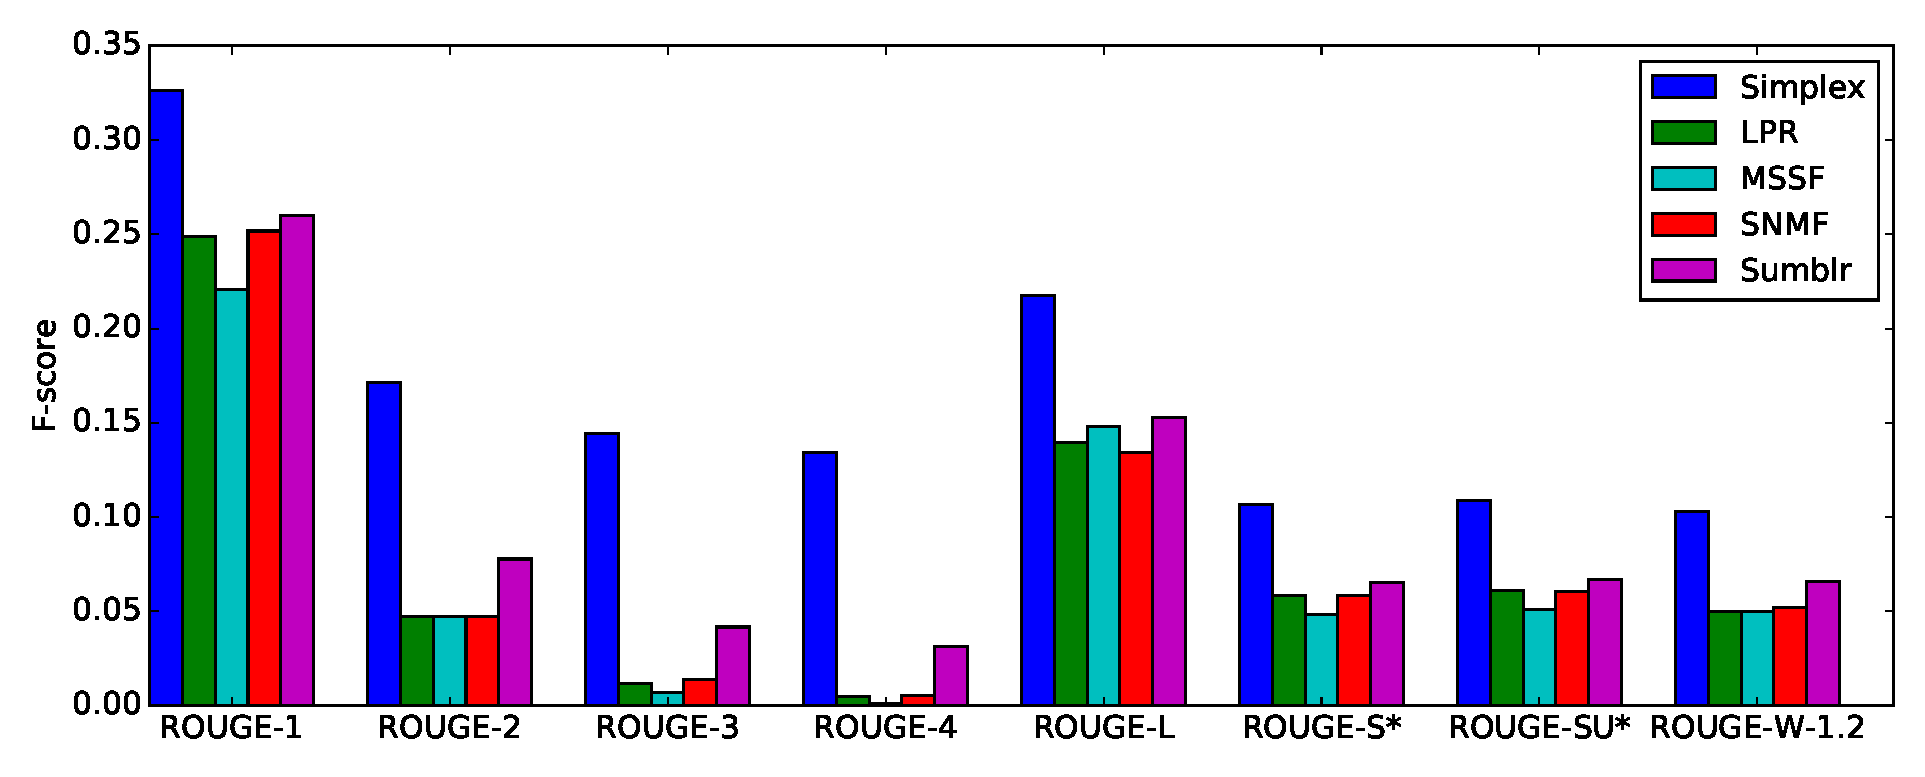
\includegraphics[scale=0.6]{rouge.eps}

\end{figure}

\begin{table}[htp]\label{table:update 0f simplex}
\caption{the updateRatio of Simplex}
\begin{center}
\begin{tabular}{|c|c|c|c|}
    \hline
    Event & Time1 & Time2 & Time3 \\
    \hline
    EOutbreak & 0 & 0.57 & 0.38 \\
    \hline
    GUattack & 0 & 0.36 & 0.33 \\
    \hline
    HProtest & 0.38 & 0.67 & 0.96 \\
    \hline
    THagupit & 0 & 0.1 & 0.62\\
    \hline
    CHShoot & 0.94 & 0.62 & 0.25\\
    \hline
    HPatricia & 0 & 0.75 & 0.83\\
    \hline
    RWelcome & 0.20 & 0.50 & 0\\
    \hline
    BAExplossion & 1 & 0.67 & 0.80\\
    \hline
    HPCyprus & 0.88 & 0.65 & 0.76\\
    \hline
    LBlast & 0.22 & 0.50 & 0.69\\
    \hline
\end{tabular}
\end{center}
\label{default}
\end{table}

\begin{table}[htp]\label{table:update 0f sumblr}
\caption{the updateRatio of Sumblr}
\begin{center}
\begin{tabular}{|c|c|c|c|}
    \hline
    Event & Time1 & Time2 & Time3 \\
    \hline
    EOutbreak & 0.75 & 0.30 & 0.20 \\
    \hline
    GUattack & 0.65 & 0.50 & 0.30 \\
    \hline
    HProtest & 0.35 & 0.40 & 0.30 \\
    \hline
    THagupit & 0.65 & 0.45 & 0.10\\
    \hline
    CHShoot & 0.20 & 0.05 & 0.10\\
    \hline
    HPatricia & 0.25 & 0.20 & 0\\
    \hline
    RWelcome & 0.35 & 0.35 & 0.20\\
    \hline
    BAExplossion & 0.45 & 0.35 & 0\\
    \hline
    HPCyprus & 0.30 & 0.15 & 0.25\\
    \hline
    LBlast & 0.30 & 0.25 & 0.05\\
    \hline
\end{tabular}
\end{center}
\label{default}
\end{table}

\begin{table}[htp]\label{table:update 0f mssf}
\caption{the updateRatio of MSSF}
\begin{center}
    \begin{tabular}{|c|c|c|c|}
    \hline
    Event & Time1 & Time2 & Time3 \\
    \hline
    EOutbreak & 0.41 & 0.29 & 0.24 \\
    \hline
    GUattack & 0.62 & 0.18 & 0.18 \\
    \hline
    HProtest & 0.65 & 0.22 & 0.17 \\
    \hline
    THagupit & 0.39 & 0.61 & 0.18\\
    \hline
    CHShoot & 0.33 & 0.39 & 0.18\\
    \hline
    HPatricia & 0.47 & 0.29 & 0\\
    \hline
    RWelcome & 0.44 & 0.62 & 0.17\\
    \hline
    BAExplossion & 0.39 & 0.12 & 0.12\\
    \hline
    HPCyprus & 0.11 & 0.17 & 0.17\\
    \hline
    LBlast & 0.35 & 0.50 & 0.33\\
    \hline
    \end{tabular}
\end{center}
\label{default}
\end{table}

\subsection{Inconsistency Detection Performance}
%comparative methods
In addition of the state-of-the-art summarization methods, for comparison on inconsistency detection, we adopted some naive methods

%result table or figure
\begin{table*}
\begin{floatrow}
\capbtabbox{
    \begin{tabular}{|c|c|c|c|c|}
    \hline
    Event & Time0 & Time1 & Time2 & Time3 \\
    \hline
    EOutbreak & 0.65 & 0.70 & 0.65 & 0.70 \\
    \hline
    GUattack & 0.60 & 0.55 & 0.40 & 0.50 \\
    \hline
    HProtest & 0.60 & 0.55 & 0.55 & 0.50 \\
    \hline
    THagupit & 0.70 & 0.75 & 0.70 & 0.65\\
    \hline
    CHShoot & 0.85 & 0.70 & 0.75 & 0.70\\
    \hline
    HPatricia & 0.75 & 0.75 & 0.75 & 0.75\\
    \hline
    RWelcome & 0.65 & 0.60 & 0.65 & 0.65\\
    \hline
    BAExplossion & 0.80 & 0.60 & 0.60 & 0.55\\
    \hline
    HPCyprus & 0.50 & 0.55 & 0.55 & 0.55\\
    \hline
    LBlast & 0.65 & 0.60 & 0.55 & 0.55\\
    \hline
    \end{tabular}
    }{
    \caption{the inconsistency of Sumblr}
    \label{table:inconsistency 0f Sumblr}
}

\capbtabbox{
    \begin{tabular}{|c|c|c|c|c|}
    \hline
    Event & Time0 & Time1 & Time2 & Time3 \\
    \hline
    EOutbreak & 0.76 & 0.71 & 0.76 & 0.78 \\
    \hline
    GUattack & 0.62 & 0.59 & 0.59 & 0.47 \\
    \hline
    HProtest & 0.27 & 0.33 & 0.44 & 0.44 \\
    \hline
    THagupit & 0.83 & 0.83 & 0.82 & 0.82\\
    \hline
    CHShoot & 0.83 & 0.78 & 0.76 & 0.71\\
    \hline
    HPatricia & 0.71 & 0.71 & 0.76 & 0.76\\
    \hline
    RWelcome & 0.69 & 0.75 & 0.72 & 0.72\\
    \hline
    BAExplossion & 0.67 & 0.71 & 0.76 & 0.83\\
    \hline
    HPCyprus & 0.83 & 0.89 & 0.72 & 0.65\\
    \hline
    LBlast & 0.41 & 0.56 & 0.50 & 0.56\\
    \hline
    \end{tabular}
    }{
    \caption{the inconsistency of MSSF}
    \label{table:inconsistency 0f MSSF}
}
\end{floatrow}
\end{table*}

\begin{table}[htp]\label{table:inconsistency 0f others}
\caption{the inconsistency of others}
\begin{center}
\begin{tabular}{|c|c|c|}
    \hline
    Event & SNMF & LPR \\
    \hline
    EOutbreak & 0.67 & 0.80 \\
    \hline
    GUattack & 0.47 & 0.40 \\
    \hline
    HProtest & 0.20 & 0.10 \\
    \hline
    THagupit & 0.33 & 0.20\\
    \hline
    CHShoot & 0.60 & 0.60\\
    \hline
    HPatricia & 0.53 & 0.50\\
    \hline
    RWelcome & 0.33 & 0.20\\
    \hline
    BAExplossion & 0.33 & 0.30\\
    \hline
    HPCyprus & 0.33 & 0.30\\
    \hline
    LBlast & 0.07 & 0.10\\
    \hline
\end{tabular}
\end{center}
\label{default}
\end{table}

\subsection{Efficiency Study}

%goal

%result figure

\begin{figure}
    \centering
    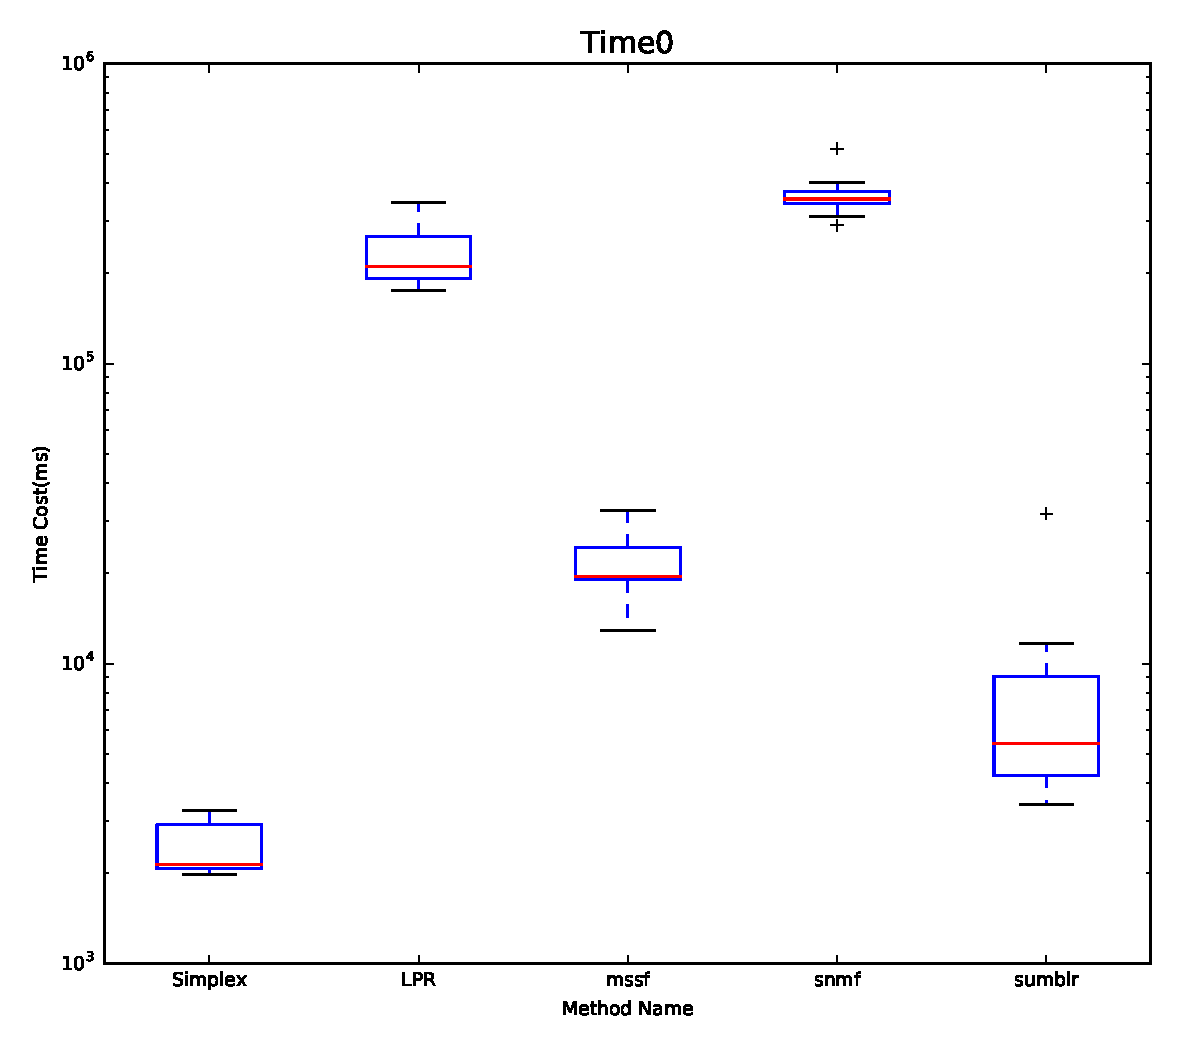
\includegraphics[scale=0.5]{log_time0.eps}

    \label{fig:side:a}
\end{figure}

\begin{figure}
    \centering
    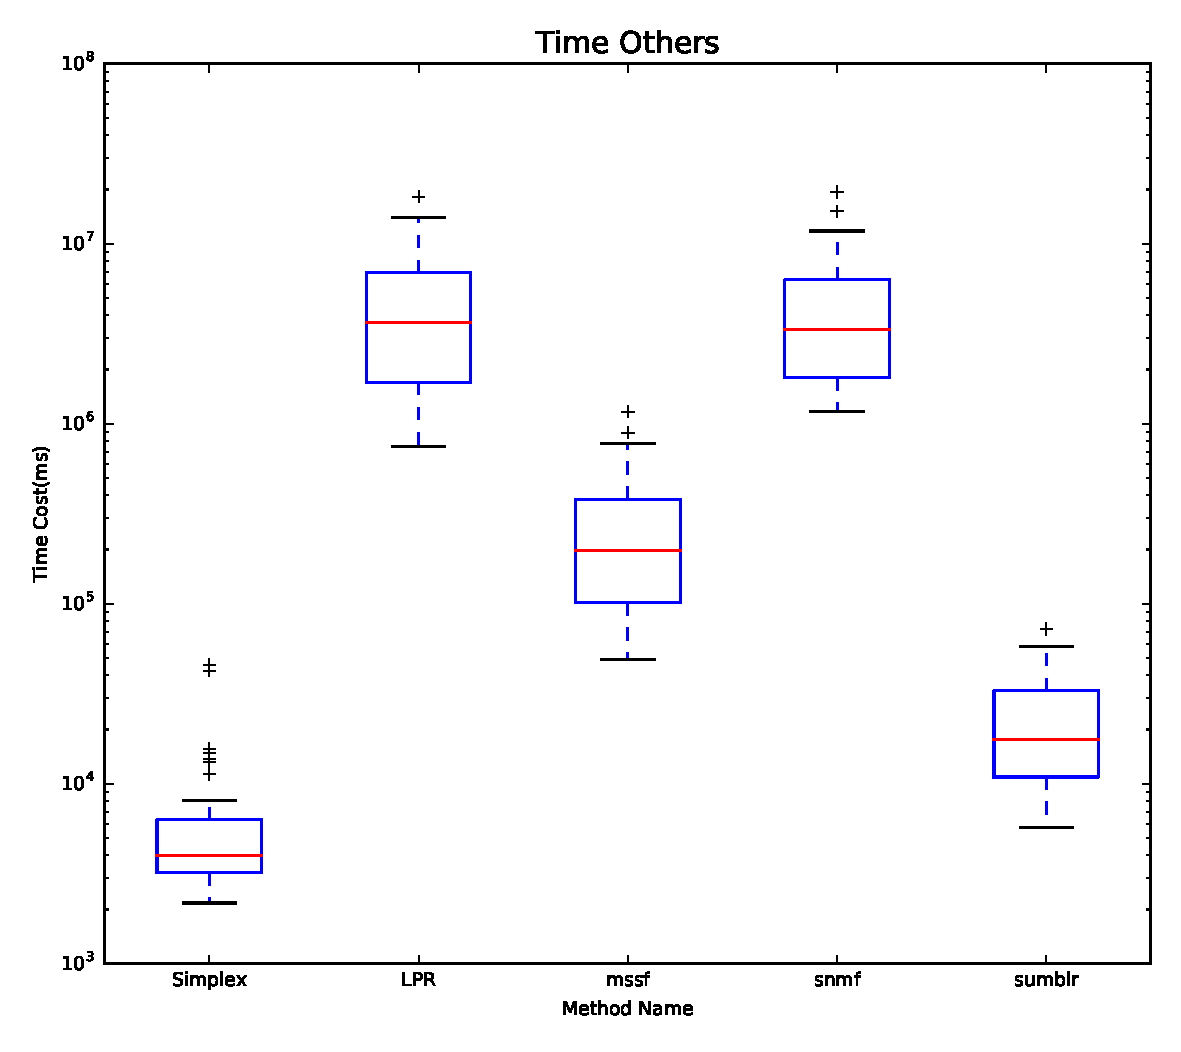
\includegraphics[scale=0.5]{log_time1.eps}
    \caption{fig2}
    \label{fig:side:b}
\end{figure}

\subsection{Effects of Parameters}

%goal

%result figure
\begin{figure}
    \centering
    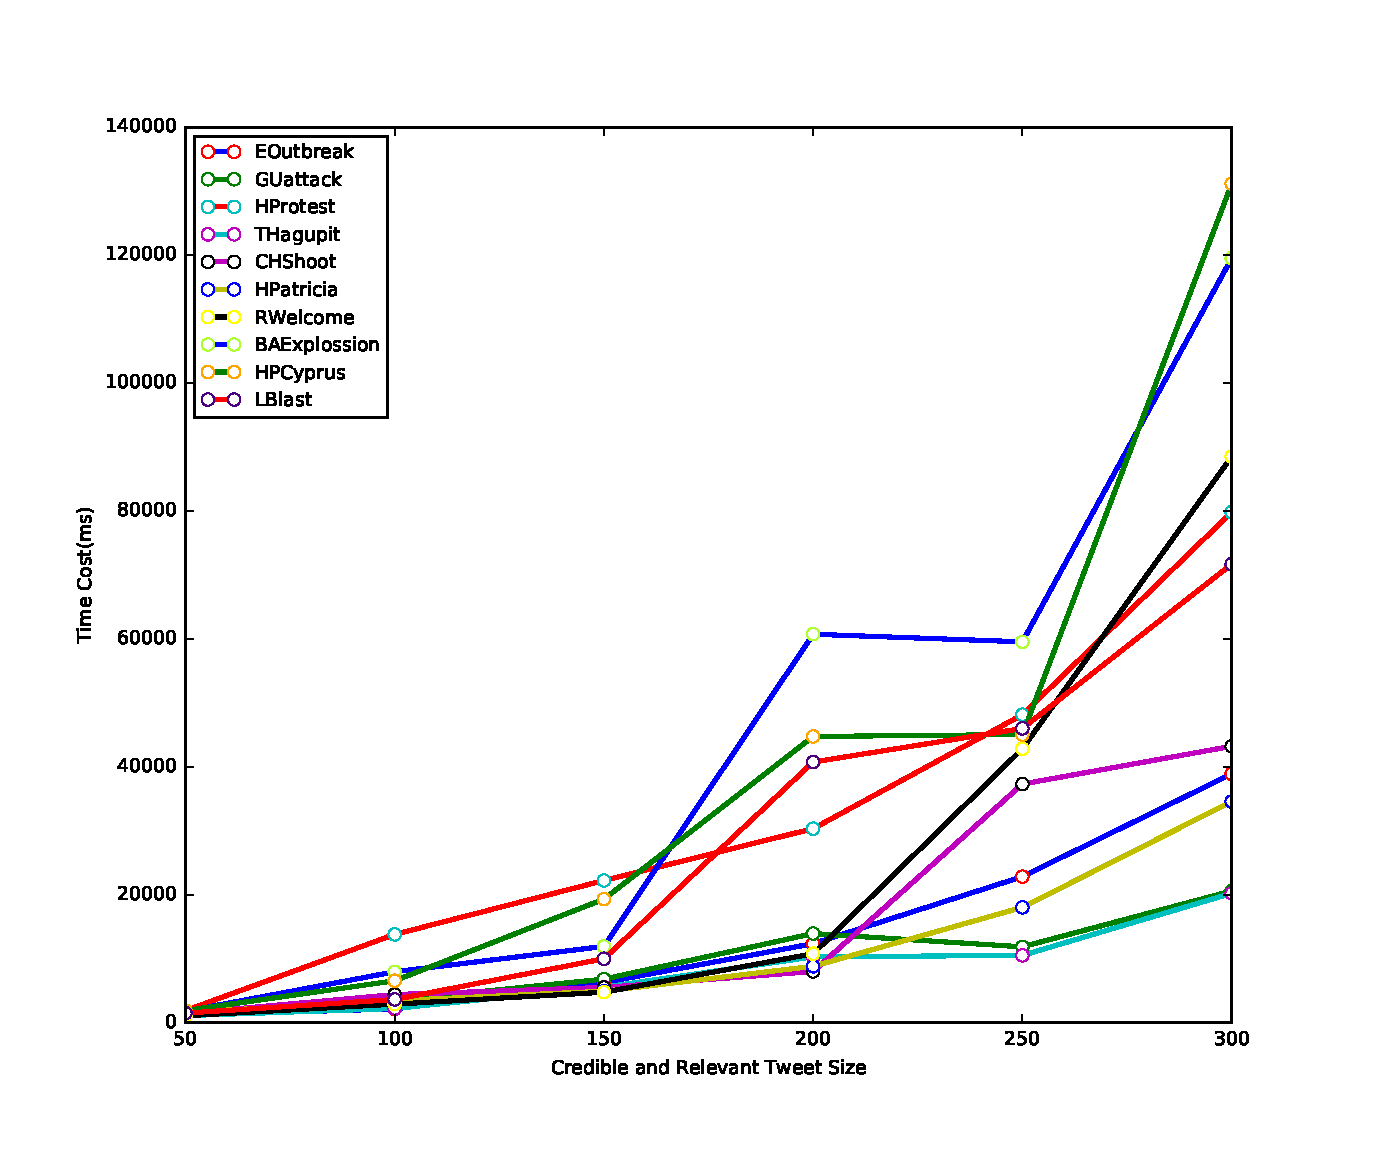
\includegraphics[scale=0.5]{summary-timecost.eps}

\end{figure}

\begin{figure}
    \centering
    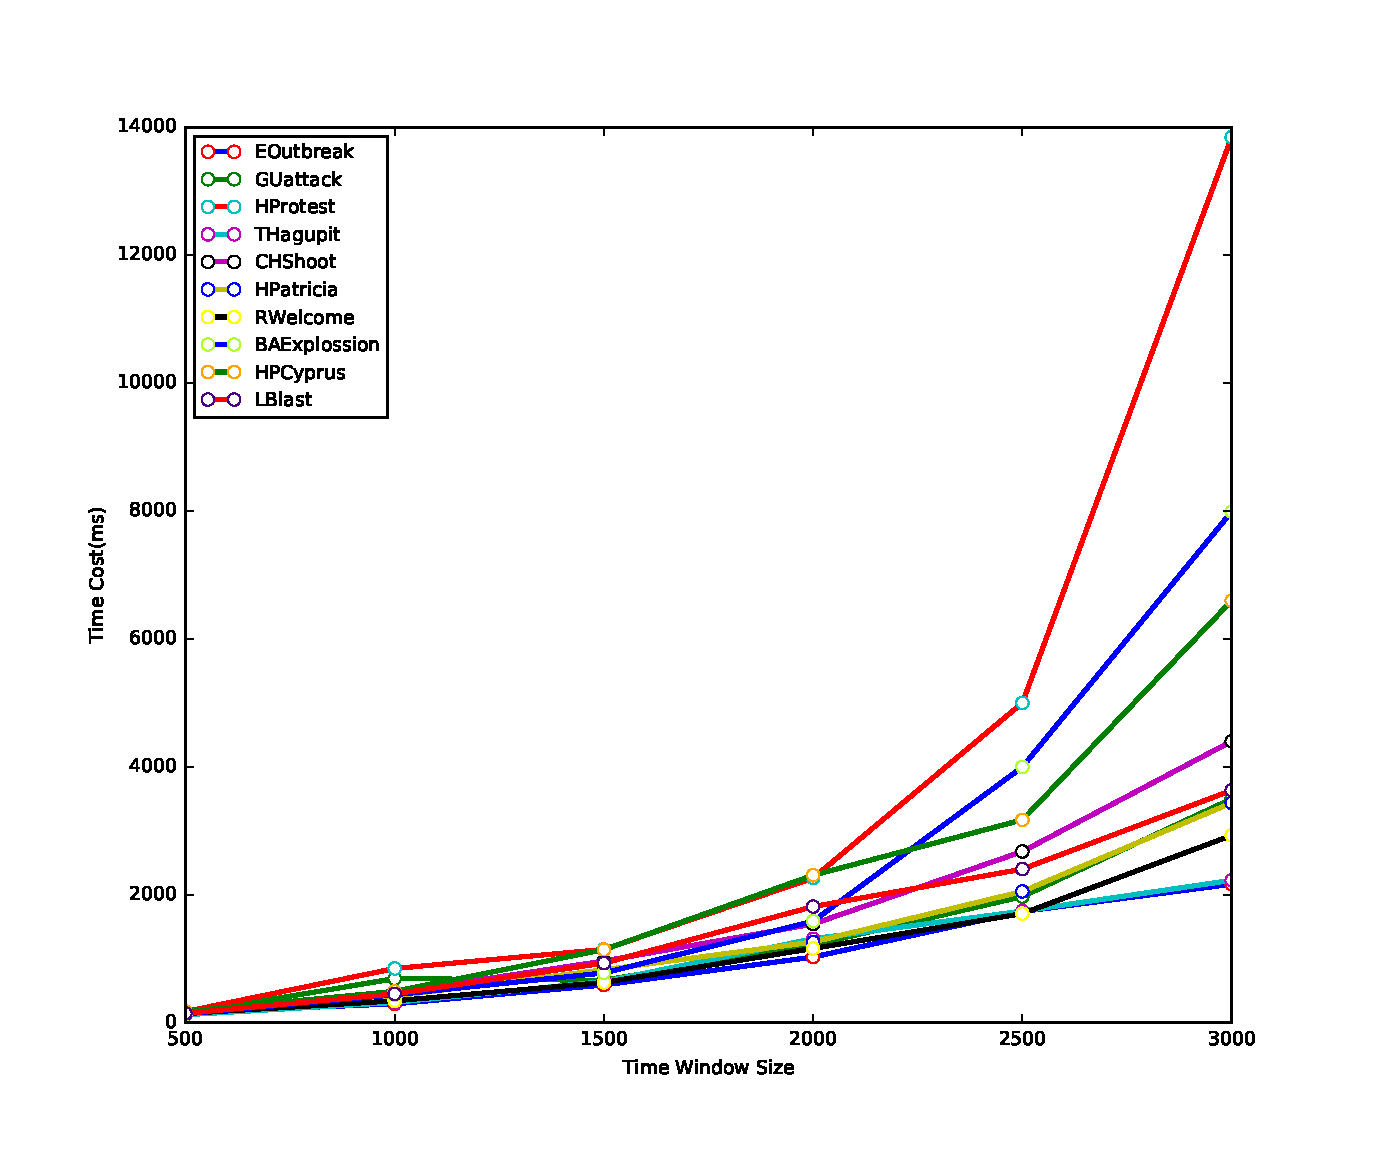
\includegraphics[scale=0.5]{window-timecost.eps}

\end{figure}

\section{Conclusion}\label{sec:conclusion}
\begin{thebibliography}{10}

\bibitem{Chin2017TOTEM}
J.~Y. Chin, S.~S. Bhowmick, and A.~Jatowt.
\newblock Totem: Personal tweets summarization on mobile devices.
\newblock In {\em Proceedings of the 40th International ACM SIGIR Conference on
  Research and Development in Information Retrieval}, SIGIR '17, pages
  1305--1308, New York, NY, USA, 2017. ACM.

\bibitem{Efron2011Estimation}
M.~Efron and G.~Golovchinsky.
\newblock Estimation methods for ranking recent information.
\newblock In {\em Proceedings of the 34th international ACM SIGIR conference on
  Research and development in Information}, SIGIR '11, pages 495--504, New
  York, NY, USA, 2011. ACM.

\bibitem{Gillani2017Post}
M.~Gillani, M.~U. Ilyas, S.~Saleh, J.~S. Alowibdi, N.~Aljohani, and F.~S.
  Alotaibi.
\newblock Post summarization of microblogs of sporting events.
\newblock In {\em Proceedings of the 26th International Conference on World
  Wide Web Companion}, WWW '17 Companion, pages 59--68, Republic and Canton of
  Geneva, Switzerland, 2017. International World Wide Web Conferences Steering
  Committee.

\bibitem{Hannon2010Recommending}
J.~Hannon, M.~Bennett, and B.~Smyth.
\newblock Recommending twitter users to follow using content and collaborative
  filtering approaches.
\newblock In {\em Proceedings of the fourth ACM conference on Recommender
  systems}, RecSys '10, pages 199--206, New York, NY, USA, 2010. ACM.

\bibitem{kwak2010twitter}
H.~Kwak, C.~Lee, H.~Park, and S.~Moon.
\newblock What is twitter, a social network or a news media?
\newblock In {\em Proceedings of the 19th international conference on World
  wide web}, pages 591--600. ACM, 2010.

\bibitem{Lin2012Generating}
C.~Lin, C.~Lin, J.~Li, D.~Wang, Y.~Chen, and T.~Li.
\newblock Generating event storylines from microblogs.
\newblock In {\em Proceedings of the 21st ACM international conference on
  Information and knowledge management}, CIKM '12, pages 175--184, New York,
  NY, USA, 2012. ACM.

\bibitem{Liu2016LEDS}
Z.~Liu, Y.~Huang, and J.~R. Trampier.
\newblock Leds: Local event discovery and summarization from tweets.
\newblock In {\em Proceedings of the 24th ACM SIGSPATIAL International
  Conference on Advances in Geographic Information Systems}, GIS '16, pages
  53:1--53:4, New York, NY, USA, 2016. ACM.

\bibitem{Mathioudakis2010TwitterMonitor}
M.~Mathioudakis and N.~Koudas.
\newblock Twittermonitor: trend detection over the twitter stream.
\newblock In {\em Proceedings of the 2010 international conference on
  Management of data}, SIGMOD '10, pages 1155--1158, New York, NY, USA, 2010.
  ACM.

\bibitem{Meng2012Entitycentric}
X.~Meng, F.~Wei, X.~Liu, M.~Zhou, S.~Li, and H.~Wang.
\newblock Entity-centric topic-oriented opinion summarization in twitter.
\newblock In {\em Proceedings of the 18th ACM SIGKDD international conference
  on Knowledge discovery and data mining}, KDD '12, pages 379--387, New York,
  NY, USA, 2012. ACM.

\bibitem{Ren2013Personalized}
Z.~Ren, S.~Liang, E.~Meij, and M.~de~Rijke.
\newblock Personalized time-aware tweets summarization.
\newblock In {\em Proceedings of the 36th international ACM SIGIR conference on
  Research and development in information retrieval}, SIGIR '13, pages
  513--522, New York, NY, USA, 2013. ACM.

\bibitem{Lin2008Storyline-based}
F.~ren Lin and C.-H. Liang.
\newblock Storyline-based summarization for news topic retrospection.
\newblock {\em Decision Support Systems}, 45(3):473 -- 490, 2008.
\newblock <ce:title>Special Issue Clusters</ce:title>.

\bibitem{Rudra2016Summarizing}
K.~Rudra, S.~Banerjee, N.~Ganguly, P.~Goyal, M.~Imran, and P.~Mitra.
\newblock Summarizing situational tweets in crisis scenario.
\newblock In {\em Proceedings of the 27th ACM Conference on Hypertext and
  Social Media}, HT '16, pages 137--147, New York, NY, USA, 2016. ACM.

\bibitem{Rudra2015Extracting}
K.~Rudra, S.~Ghosh, N.~Ganguly, P.~Goyal, and S.~Ghosh.
\newblock Extracting situational information from microblogs during disaster
  events: A classification-summarization approach.
\newblock In {\em Proceedings of the 24th ACM International on Conference on
  Information and Knowledge Management}, CIKM '15, pages 583--592, New York,
  NY, USA, 2015. ACM.

\bibitem{Sharifi2010Summarizing}
B.~Sharifi, M.-A. Hutton, and J.~Kalita.
\newblock Summarizing microblogs automatically.
\newblock In {\em Human Language Technologies: The 2010 Annual Conference of
  the North American Chapter of the Association for Computational Linguistics},
  HLT '10, pages 685--688, Stroudsburg, PA, USA, 2010. Association for
  Computational Linguistics.

\bibitem{Shou2013Sumblr}
L.~Shou, Z.~Wang, K.~Chen, and G.~Chen.
\newblock Sumblr: continuous summarization of evolving tweet streams.
\newblock In {\em Proceedings of the 36th international ACM SIGIR conference on
  Research and development in information retrieval}, SIGIR '13, pages
  533--542, New York, NY, USA, 2013. ACM.

\bibitem{Takamura2011Summarizing}
H.~Takamura, H.~Yokono, and M.~Okumura.
\newblock Summarizing a document stream.
\newblock In {\em Proceedings of the 33rd European conference on Advances in
  information retrieval}, ECIR'11, pages 177--188, Berlin, Heidelberg, 2011.
  Springer-Verlag.

\bibitem{Wang2009Evolutionary}
D.~Wang, L.~Zheng, T.~Li, and Y.~Deng.
\newblock Evolutionary document summarization for disaster management.
\newblock In {\em Proceedings of the 32nd international ACM SIGIR conference on
  Research and development in information retrieval}, pages 680--681. ACM,
  2009.

\bibitem{Yan2011Evolutionary}
R.~Yan, X.~Wan, J.~Otterbacher, L.~Kong, X.~Li, and Y.~Zhang.
\newblock Evolutionary timeline summarization: a balanced optimization
  framework via iterative substitution.
\newblock In {\em Proceedings of the 34th international ACM SIGIR conference on
  Research and development in Information}, pages 745--754. ACM, 2011.

\bibitem{Yih2007Multi-document}
W.~Yih, J.~Goodman, L.~Vanderwende, and H.~Suzuki.
\newblock Multi-document summarization by maximizing informative content-words.
\newblock In {\em Proceedings of IJCAI}, volume~7, 2007.

\bibitem{Zubiaga2012Towards}
A.~Zubiaga, D.~Spina, E.~Amig\'{o}, and J.~Gonzalo.
\newblock Towards real-time summarization of scheduled events from twitter
  streams.
\newblock In {\em Proceedings of the 23rd ACM conference on Hypertext and
  social media}, HT '12, pages 319--320, New York, NY, USA, 2012. ACM.

\end{thebibliography}


\end{document}
